\section{PoseGraph SLAM}

Consider the problem of full SLAM: 
\begin{figure}[H]
    \centering
    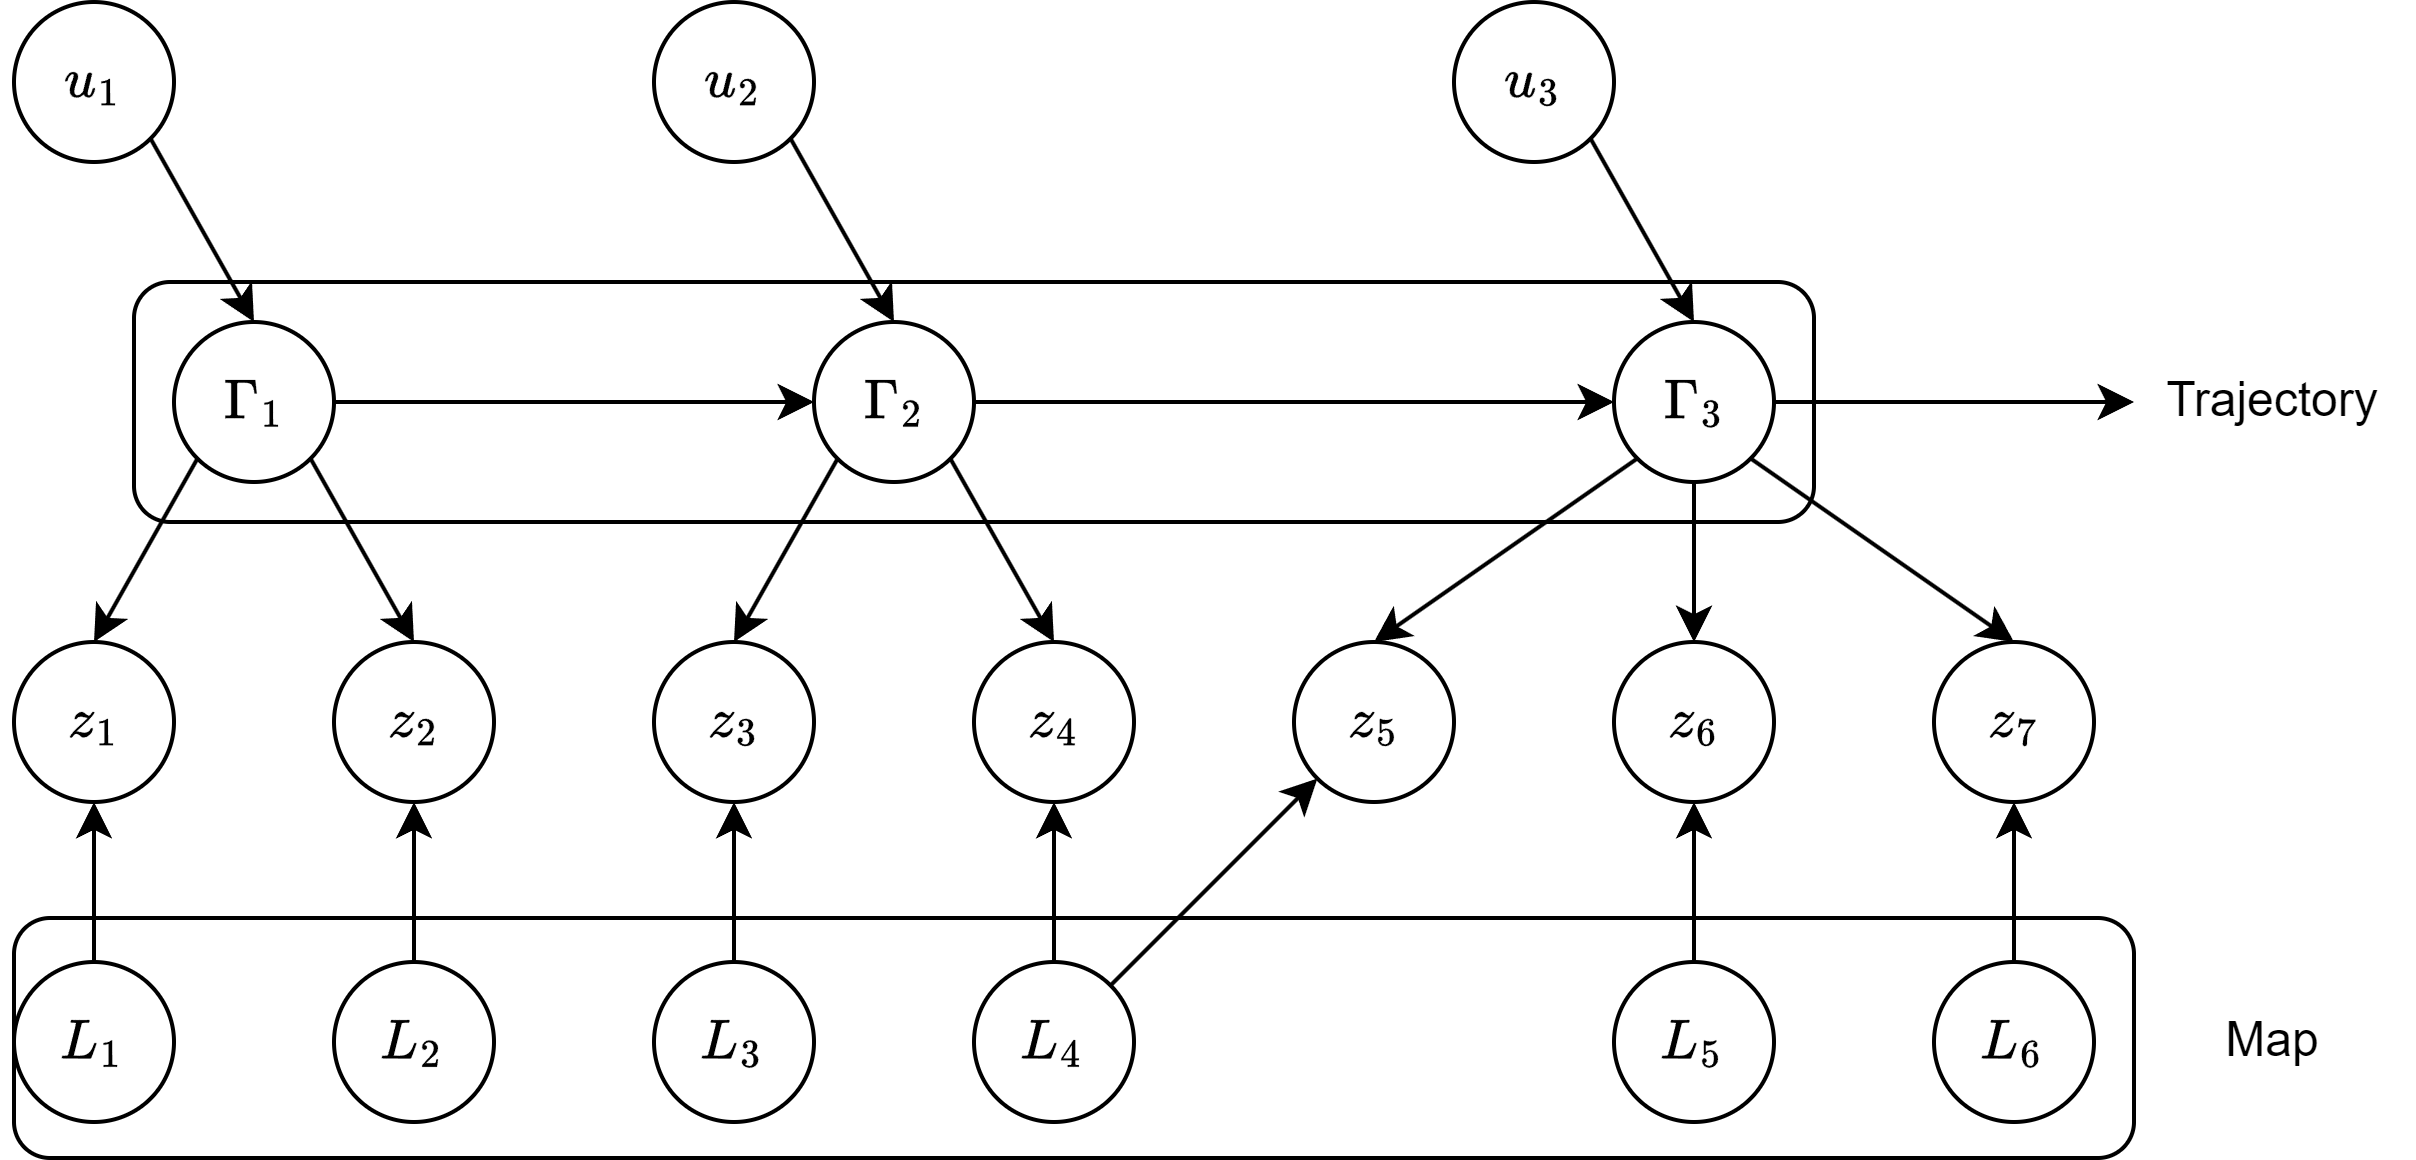
\includegraphics[width=0.75\linewidth]{images/slam.png}
    \caption{Simultaneous Localization and Mapping}
\end{figure}
In Full SLAM we model: 
\[\Pr(X|Z,U)=\Pr(\Gamma_{0:t},L_1,\ldots,L_n|z_{1:t},u_{1:t})\]
then we look for the most likely solution
\[X^{MAP}=\argmax_X\Pr(X|Z,U)\]
This can be rewritten using the Bayes' rule as
\[X^{MAP}=\argmax_X\Pr(X,Z,U)\]
The maximum of this probability will be located in the same spot of the previous, since the denominator is only a normalizing factor and do not depends on $X$. 

The full joint distribution of a Bayesian network is the product of the conditionals: 
\begin{multline*}
    \Pr(X,Z,U)=\Pr(\Gamma_{0:3},L_1,\ldots,L_6 Z_{1:7},u_{1:7})= 
    \Pr(\Gamma_1|\Gamma_0,u_{1})
    \Pr(\Gamma_2|\Gamma_1,u_{1})
    \Pr(\Gamma_3|\Gamma_2,u_{3}) \\
    \Pr(Z_1|\Gamma_1,L_1)
    \Pr(L_1)
    \Pr(Z_2|\Gamma_1,L_2)
    \Pr(L_2)
    \Pr(Z_3|\Gamma_2,L_3)
    \Pr(L_3) \\
    \Pr(Z_4|\Gamma_2,L_4)
    \Pr(L_4)
    \Pr(Z_5|\Gamma_3,L_4)
    \Pr(Z_6|\Gamma_3,L_5)
    \Pr(L_5)
    \Pr(Z_7|\Gamma_3,L_6)
    \Pr(L_6)
\end{multline*}
By using the Bayes' rule we obtain that it is the product of factors: 
\begin{multline*}
    \Pr(X,Z,U)=
    \phi(\Gamma_1,\Gamma_0,u_{1})
    \phi(\Gamma_2,\Gamma_1,u_{1})
    \phi(\Gamma_3,\Gamma_2,u_{3}) \\
    \phi(Z_1,\Gamma_1,L_1)
    \phi(L_1)
    \phi(Z_2,\Gamma_1,L_2)
    \phi(L_2)
    \phi(Z_3,\Gamma_2,L_3)
    \phi(L_3) \\
    \phi(Z_4,\Gamma_2,L_4)
    \phi(L_4)
    \phi(Z_5,\Gamma_3,L_4)
    \phi(Z_6,\Gamma_3,L_5)
    \phi(L_5)
    \phi(Z_7,\Gamma_3,L_6)
    \phi(L_6)
\end{multline*}
At this point the Bayesian Network becomes: 
\begin{figure}[H]
    \centering
    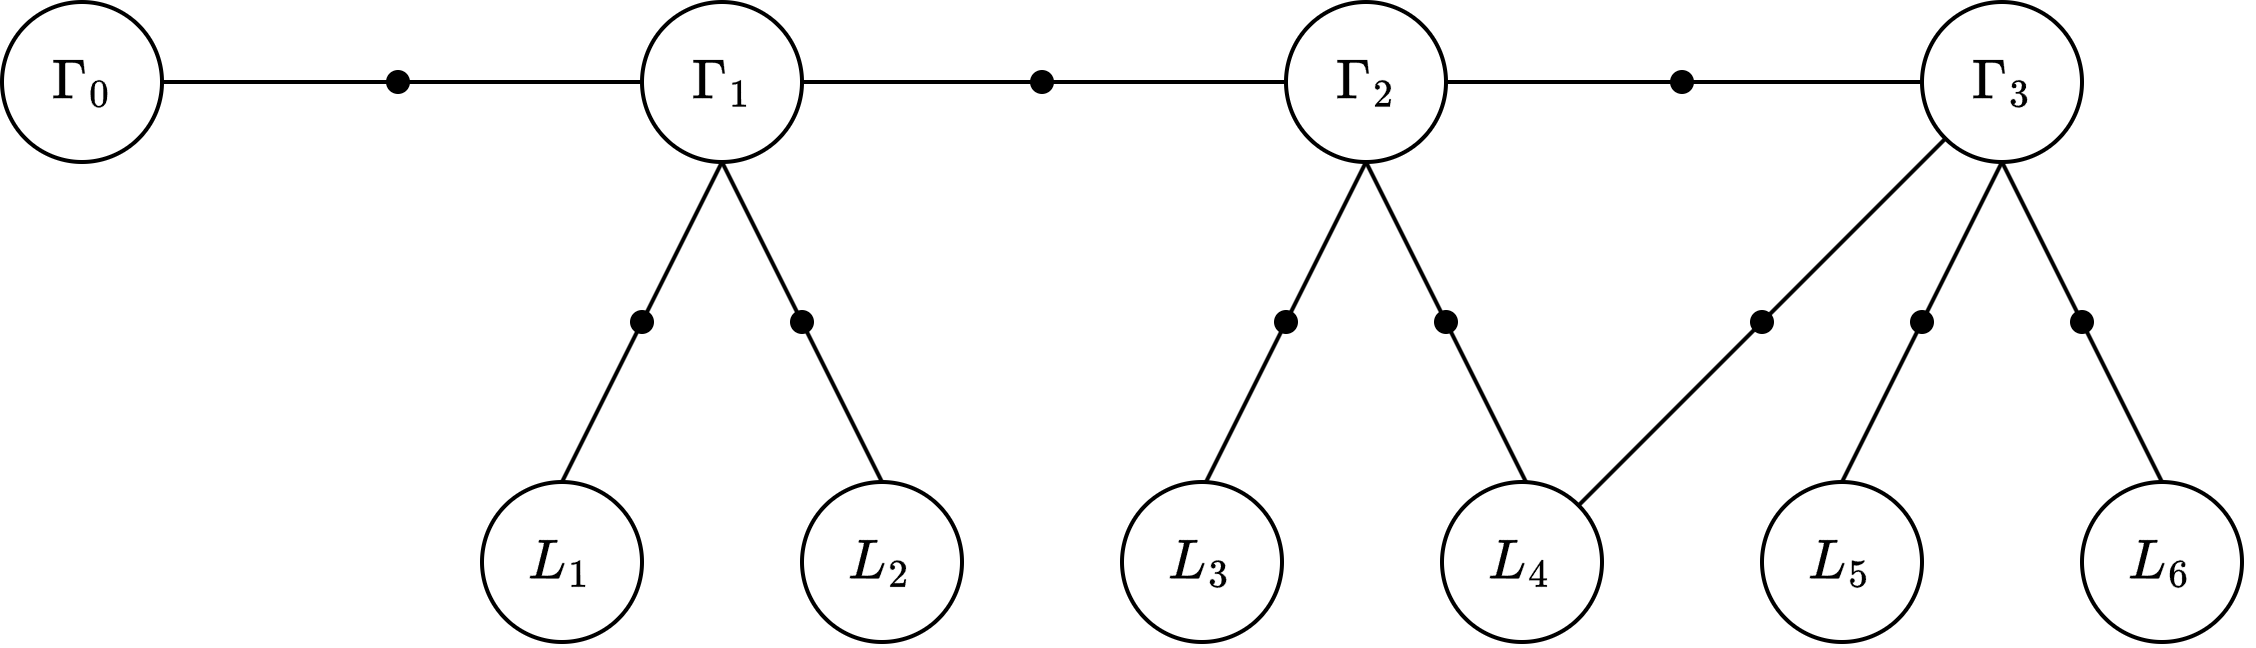
\includegraphics[width=0.75\linewidth]{images/facslam.png}
    \caption{Factorized Simultaneous Localization and Mapping}
\end{figure}
Given the Factor Graph Full Joint Distribution: 
\[\Pr(X,Z,U)=\prod_i\phi_i(X_i)\]
The Full SLAM problem is reformulated as
\[X^{MAP}=\argmax_X\Pr(X|Z,U)=\argmax_X\Pr(X,Z,U)=\argmax_X\prod_i\phi_i(X_i)\]
Let's also assume to have Gaussian Factors (not mandatory but convenient): 
\[\phi(\Gamma_1, \Gamma_0, u_1)= \mathcal{N}(g(\Gamma_0,u_1),R) =\dfrac{1}{\sqrt{\left\lvert 2\pi R\right\rvert}}e^{-\frac{1}{2}(g(\Gamma_0,u_1)-\Gamma_1)^TR^{-1}(g(\Gamma_0,u_1)-\Gamma_1)}\]
\[\phi(Z_1, \Gamma_1, L_1)= \mathcal{N}(h(\Gamma_1,L_1),Q) =\dfrac{1}{\sqrt{\left\lvert 2\pi Q\right\rvert}}e^{-\frac{1}{2}(h(\Gamma_1,L_1)-Z_1)^TQ^{-1}(h(\Gamma_1,L_1)-Z_1)}\]
The Odometry factors are proportional to the exponential: 
\[\phi_{i=u_i}\propto e^{-\frac{1}{2}(g_i(X_i)-\Gamma_i)^TR^{-1}(g_i(X_i)-\Gamma_i)}\]
The measurement factors are proportional to the exponential: 
\[\phi_{i=z_i}\propto e^{-\frac{1}{2}(h_i(X_i)-Z_i)^TQ^{-1}(h_i(X_i)-Z_i)}\]
The (Gaussian) Full SLAM problem becomes: 
\begin{align*}
    X^{MAP} &=\argmax_{X}=\prod_i\phi_i(X_i)=\argmax_{X} \\
            &=\prod_ie^{-\frac{1}{2}(g_i(X_i)-\Gamma_i)^TR^{-1}(g_i(X_i)-\Gamma_i)}\prod_ie^{-\frac{1}{2}(h_i(X_i)-Z_i)^TQ^{-1}(h_i(X_i)-Z_i)}
\end{align*}
If we solve for the logarithm we get a simpler optimization algorithm: 
\begin{align*}
    X^{MAP} &=\argmax_X\prod_i\phi_i(X_i)=\argmax_X\log\prod_i\phi_i(X_i)=\argmax_X\sum_i\log\phi_i(X_i)\\
            &=\argmax_X\left[\sum_{i=u_i}\log\left(e^{-\frac{1}{2}\left\lVert g_i(X_i)-\Gamma_i\right\rVert _R^2}\right)+\sum_{i=z_i}\log\left(e^{-\frac{1}{2}\left\lVert h_i(X_i)-Z_i\right\rVert _Q^2}\right)\right] \\
            &=\argmax_X\left[\sum_{i=u_i}\left(-\dfrac{1}{2}\left\lVert g_i(X_i)-\Gamma_i\right\rVert _R^2\right)+\sum_{i=z_i}\left(-\frac{1}{2}\left\lVert h_i(X_i)-Z_i\right\rVert _Q^2\right)\right] \\
            &=\argmin_X\left[\sum_{i=u_i}\left\lVert g_i(X_i)-\Gamma_i\right\rVert _R^2 +\sum_{i=z_i}\left\lVert h_i(X_i)-Z_i\right\rVert _Q^2\right] 
\end{align*}
That is the nonlinear least squares on a graph. 
Sometimes landmarks get attached to poses in PoseGraph SLAM.

\subsection{Computational complexity}
Solving non-linear least squares needs iterative adjustments (gradient descend). 

\paragraph*{Measurement factors}
Let’s focus on measurement factors, then the following extends to all factors
\[h_i(X_i)=h_i(X_i^0)+\Delta_i\approx h_i(X_i^0)+H_i\Delta_i\]
Here, $\Delta_i=X_i-X_i^0$, and $H_i$ is the Hessian computed in $X_i^0$. 
We look for the single adjustment step which minimizes all measurement factors:
\[\Delta^\ast=\argmin_{\Delta}\sum_{i=z_i}\left\lVert h_i(X_i)-Z_i\right\rVert _Q^2=\argmin_{\Delta}\sum_{i=z_i}\left\lVert \underbrace{H_i\Delta_i-\left(Z_i-h_i(X_i^0)\right)}_{e_i} \right\rVert _Q^2\]
That is equivalent to minimize the error. 
We can rewrite the Mahalanobis norm as it follows turning it into quadratic:
\[\left\lVert e_i \right\rVert _Q^2=e_i^TQe_i=\left(Q^{-\frac{1}{2}}e_i\right)^T\left(Q^{-\frac{1}{2}}e_i\right)=\left\lVert Q^{-\frac{1}{2}}e \right\rVert _2^2\]
We can now rewrite the minimization as: 
\[\Delta^\ast=\argmin_{\Delta}\sum_{i=z_i}\left\lVert Q_i^{-\frac{1}{2}}H_i\Delta_i-Q_i^{-\frac{1}{2}}\left(Z_i-h_i(X_i^0)\right) \right\rVert _2^2\]
By imposing $A_i=Q_i^{-\frac{1}{2}}H_i$ and $b_i=Q_i^{-\frac{1}{2}}\left(Z_i-h_i(X_i^0)\right)$ we get: 
\[\Delta^\ast=\argmin_{\Delta}\sum_{i=z_i}\left\lVert A_i\Delta_i-b_i \right\rVert _2^2=\argmin_{\Delta}\sum_{i=z_i}\left\lVert A\Delta-B \right\rVert _2^2\]
This is Linear least squares problem. 
Let's assume Odometry is included too from now on. 

Let’s solve the least squares problem
\[\left\lVert A\Delta-B \right\rVert _2^2=(A\Delta-B)^T(A\Delta-B)=\Delta^TA^TA\Delta-2\Delta^TA^TB+BB^T\]
Deriving for $Delta$ and imposing the derivative to zero we get: 
\[\dfrac{\partial\left\lVert A\Delta-B \right\rVert _2^2}{\partial\Delta}=0\rightarrow \Delta=A^TB(A^TA)^{-1}\]
Matrix $A$ from Odometry and Measurement Jacobians
Factors are constraints between 2 variables
Matrix $A$ is sparse and matrix $A^TA$ too
 We can use sparse methods which are fast . 

\paragraph*{COmplexity}
Naïve least squares uses pseudo inverse, however $(A^TA)^{-1}$ is $\mathcal{O}(n^3)$.
Cholesky decomposition $A^TA = R^TR$ ($R$ upper triangular) is $\mathcal{O}(n^{1.5})$ to $\mathcal{O}(n^2)$. 
Solve by forward / backward substitution and via $LDL^T$ decomposition is even faster.
\begin{figure}[H]
    \centering
    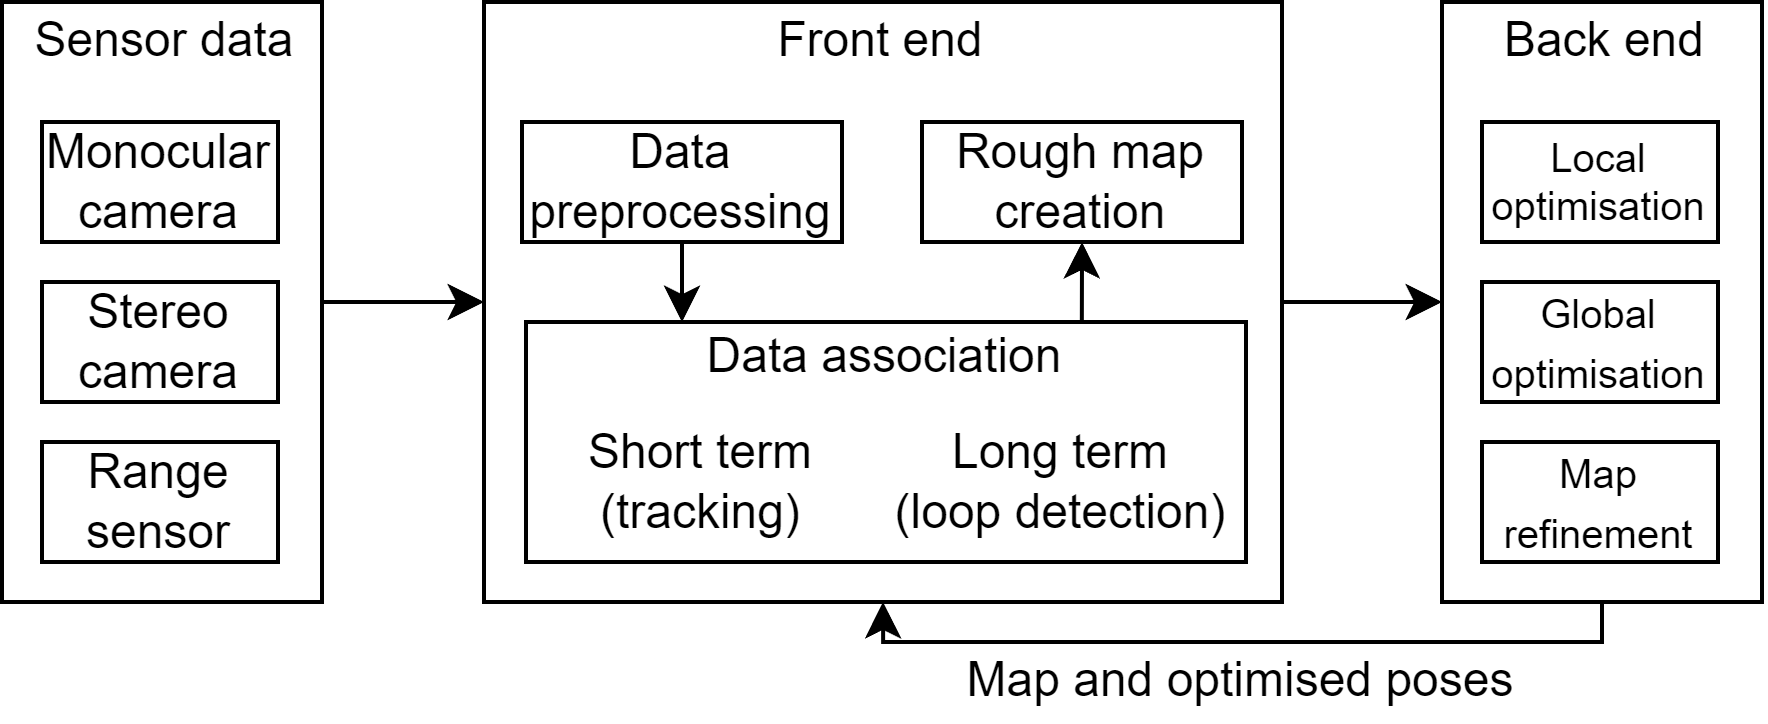
\includegraphics[width=0.75\linewidth]{images/graph.png}
    \caption{Modern SLAM System}
\end{figure}
